

\documentclass[12pt]{article}
\usepackage[utf8]{inputenc}
\usepackage[margin=1in]{geometry}
\usepackage{graphicx}
\usepackage{amsmath}
\usepackage{amsfonts}
\usepackage{amssymb}
\usepackage{booktabs}
\usepackage{listings}
\usepackage{xcolor}
\usepackage{hyperref}
\usepackage{cite}
\usepackage{fancyhdr}
\usepackage{titlesec}
\usepackage{enumitem}

% Code listing style
\lstset{
    basicstyle=\ttfamily\small,
    breaklines=true,
    frame=single,
    numbers=left,
    numberstyle=\tiny,
    showstringspaces=false,
    backgroundcolor=\color{gray!10},
    keywordstyle=\color{blue},
    commentstyle=\color{green!60!black},
    stringstyle=\color{red},
    captionpos=b
}

% Header and footer
\pagestyle{fancy}
\fancyhf{}
\rhead{Agent SME System Report}
\lhead{Major Project}
\cfoot{\thepage}

\title{\textbf{Probability SME Agent:\\
Self-Adaptive Agent Subject Matter Expert System}}


% % --- DOCUMENT INFO ---
% \title{\textbf{Probability SME Agent}}
\author{Sreemaee Akshathala \& Amey Karan \\ 
2025701028 \& 2022111026\\
Major Project Mid Eval Report}
\date{October 25, 2025}


\begin{document}

\maketitle

\begin{abstract}
This report presents a comprehensive analysis of a self-adaptive agent Subject Matter Expert (SME) system designed for processing mathematical textbooks. The system implements a dual-pipeline architecture that intelligently selects between Marker-based parsing and OCR-based processing based on document characteristics. Using the NCERT probability chapter as a proof-of-concept, the system demonstrates robust handling of complex mathematical content including LaTeX formatting, images, tables, and graphs. The implementation leverages DSPy for structured outputs, custom NER models for keyword extraction, and a hybrid RAG system for intelligent content retrieval. Key innovations include adaptive pipeline selection, metadata-rich chunking schemas, and OCR reliability optimizations inspired by the DeepSeek-OCR research.
\end{abstract}

\tableofcontents
\newpage

\section{Introduction}

Educational institutions increasingly rely on digital document processing for curriculum development and student assessment. However, mathematical textbooks pose particular challenges due to their complex notation systems, varied layouts, and integration of visual elements. Existing parsing tools struggle with preserving mathematical semantics while maintaining processing efficiency.

Our approach centers on a self-adaptive processing system that chooses between two distinct pipelines based on document characteristics. The Marker-based pipeline excels at preserving document structure and mathematical notation, while the OCR-based pipeline provides predictable token usage and handles dense layouts effectively. This dual approach allows the system to optimize both accuracy and cost depending on the specific document being processed.

\subsection{Problem Statement}

Mathematical textbooks present several technical hurdles that standard document processors cannot adequately address. Mathematical notation requires careful preservation of spatial relationships between symbols, particularly for fractions, exponents, and complex equations. Layout complexity varies dramatically between pages, with some featuring dense multi-column text while others contain large diagrams and sparse content. Additionally, different content types within textbooks serve distinct pedagogical purposes - definitions require different processing than worked examples or practice problems. Finally, the token-intensive nature of mathematical content can make large-scale processing prohibitively expensive without careful optimization.

\subsection{Research Objectives}

This project aims to create a parsing system that maintains mathematical integrity while providing cost-effective processing. The adaptive pipeline selection mechanism automatically chooses the most appropriate processing method based on content characteristics. We developed a comprehensive metadata extraction system that categorizes content by type, difficulty, and prerequisites to enable sophisticated retrieval. The resulting RAG system leverages this structured data to provide contextually relevant responses to mathematical queries. We validated our approach using the NCERT probability chapter, which contains diverse mathematical content including complex formulas, graphs, and varied pedagogical structures.

\section{Literature Review and Technical Background}

\subsection{Document Parsing Technologies}

We evaluated several document parsing technologies to understand their capabilities and limitations for mathematical content processing.

\subsubsection{Traditional PDF Parsing Tools}

PyMuPDF demonstrated poor performance on mathematical textbooks, failing to maintain document hierarchy and losing critical structural information needed for educational content. The tool could not differentiate between headings and body text, struggled with multi-column layouts, and failed to preserve spatial relationships in mathematical expressions. Tables and figures were either ignored or poorly represented.

Docling, despite its reputation for PDF data extraction, could not adequately preserve the mathematical structure needed for educational applications. While it handled basic text extraction reasonably well, complex mathematical notation was often corrupted or simplified beyond usefulness.

DocStrange showed more promise but required extensive post-processing to reconstruct mathematical meaning. The tool treated mathematical formulas as plain text, requiring additional layers of processing to restore semantic structure.

\subsubsection{Specialized OCR Solutions}

LandingAI's document transformers showed promising results for mathematical content extraction, handling complex notation better than other tools we evaluated. However, the service imposed strict limitations on the number of pages that could be processed, making it unsuitable for large-scale textbook processing. The requirement for paid access also limited its viability for our research prototype.

\subsection{DeepSeek-OCR: A Paradigm Shift}

Recent research by DeepSeek-OCR \cite{deepseek2025} fundamentally changed our understanding of OCR reliability for mathematical content. Their work demonstrated that optical character recognition could achieve remarkable compression ratios while maintaining high accuracy, particularly relevant for our token efficiency goals.

The DeepSeek approach represents text through 2D optical mapping, using a two-component architecture that combines a specialized encoder with a decoder optimized for mathematical content. Most significantly for our work, they achieved 10× compression ratios while maintaining 97\% OCR precision, effectively reducing thousands of text tokens to hundreds of vision tokens.

The reliability metrics from DeepSeek-OCR strongly supported our decision to include an OCR-based pipeline. Their results showed 97\% precision at compression ratios below 10×, which exceeded the performance of existing tools like GOT-OCR2.0 and MinerU2.0. Even at extreme 20× compression ratios, accuracy remained around 60\%, suggesting that OCR could serve as a viable fallback for dense mathematical content. The production scalability of 200,000+ pages per day on consumer hardware made this approach particularly attractive for educational applications.

These findings directly informed our dual-pipeline architecture. The predictable token usage of OCR processing addressed one of our primary concerns about cost control in large-scale document processing. For our NCERT probability textbook, OCR consistently used 888 tokens per page regardless of content density, enabling precise cost calculations. This predictability, combined with the demonstrated reliability for complex layouts, made OCR an attractive complement to traditional parsing methods.

\section{System Architecture}

\subsection{Overview}

Our system implements a self-adaptive dual-pipeline architecture as illustrated in Figure \ref{fig:pipeline}. The system intelligently routes documents through either a Marker-based pipeline or an OCR-based pipeline based on document characteristics and token efficiency considerations.

\begin{figure}[htbp]
    \centering
    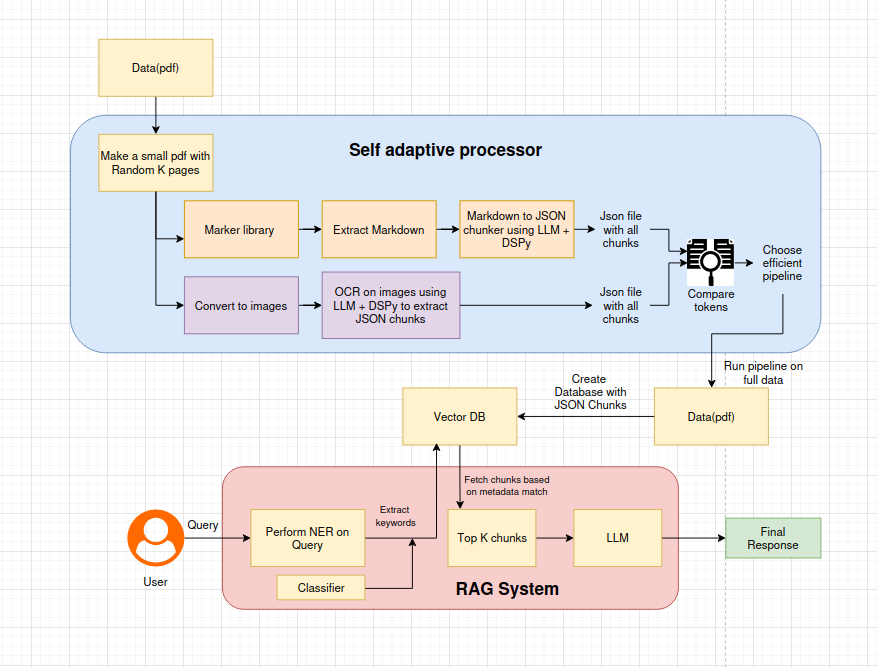
\includegraphics[width=\textwidth]{Pipeline.png}
    \caption{Self-Adaptive Agent SME System Architecture}
    \label{fig:pipeline}
\end{figure}

\subsection{Pipeline Selection Logic}

The self-adaptive processor analyzes document characteristics before selecting the optimal processing pipeline. It begins by processing a random subset of pages through both pipelines to establish baseline performance metrics. The system calculates the average token consumption for the Marker pipeline and compares this against the OCR pipeline's consistent 888-token usage per page. Based on this analysis, the processor routes the entire document through whichever pipeline offers better efficiency for that specific content type.

\subsection{Component Architecture}

The Marker-based pipeline processes PDFs directly through the Marker library, which excels at preserving document structure and mathematical notation in LaTeX format. This approach maintains hierarchical relationships and extracts images separately, making it ideal for well-structured documents with moderate content density. However, token consumption varies significantly depending on mathematical complexity and layout density.

The OCR-based pipeline converts PDF pages to images before processing them through Gemini 2.5 Flash with DSPy for structured extraction. This approach provides predictable token usage regardless of content density, making cost estimation straightforward. The pipeline handles dense multi-column layouts effectively but may introduce OCR errors depending on image quality and mathematical notation complexity.

\section{Data Collection and Preprocessing}

\subsection{Dataset Selection}

The NCERT Class 12 Probability chapter served as our proof-of-concept dataset due to its combination of mathematical complexity and pedagogical structure. This textbook contains diverse mathematical notation including probability formulas, conditional statements, and statistical expressions that test our parsing capabilities. The chapter includes various visual elements such as probability trees, statistical graphs, and tables that challenge image extraction systems. Layout complexity varies throughout the chapter, with some pages featuring dense multi-column text while others contain large diagrams with minimal accompanying text.

It is important to note that this single textbook represents only a focused proof-of-concept rather than the complete data foundation for our system. We deliberately chose to build our core architecture using a well-understood dataset to establish the fundamental processing pipelines for this mid-term submission. The goal was to create a robust foundation that demonstrates the technical feasibility of our dual-pipeline approach before scaling to larger, more diverse educational corpora.

\subsection{Marker Library Implementation}

The Marker library\footnote{\url{https://github.com/datalab-to/marker}} emerged as our preferred parsing solution after evaluating multiple alternatives. Its open-source nature allowed us to experiment extensively without licensing constraints, while the comprehensive documentation enabled rapid integration into our pipeline. Most importantly for mathematical content, Marker preserves LaTeX formatting and extracts images as separate files rather than embedded descriptions. The library offers several configuration options, including LLM-assisted parsing and forced OCR modes, which proved valuable during development and testing.

\subsection{Validation Process}

Validation required multiple verification steps to ensure processing accuracy. We tested LaTeX formula rendering by compiling extracted mathematical expressions in a standard LaTeX environment, confirming that complex probability notation remained intact. Image extraction verification involved manually checking that all graphs, diagrams, and tables were properly captured and stored separately. Content completeness checks compared processed output against the original PDF to identify any missing sections or corrupted text. Finally, we analyzed structural preservation by examining heading hierarchies, list formatting, and paragraph organization in the processed output.

\section{Chunking Schema and Metadata Design}

\subsection{Structured Schema Definition}

The chunking schema design balances comprehensive metadata capture with practical implementation constraints. Our schema structure accommodates diverse educational content types while maintaining consistency across different document sources:

\begin{lstlisting}[language=Python, caption=Chunking Schema Definition]
{
    "text": str,
    "metadata": {
        "source_url": str,
        "source_type": str,
        "topics": List[str],
        "subtopics": List[str],
        "chunk_type": Literal[
            "definition", "example", "explanation", "proof",
            "visualization", "practice_problem", "worked_solution",
            "analogy", "misconception"
        ],
        "difficulty_level": Literal["basic", "intermediate", "advanced"],
        "prerequisites": List[str]
    }
}
\end{lstlisting}

\subsection{Chunk Type Classification}

Content classification follows educational pedagogy rather than arbitrary technical categories. Definitions capture formal mathematical statements and terminology explanations. Examples provide concrete applications of abstract concepts, while explanations offer conceptual understanding through narrative description. Proofs contain logical derivations and mathematical reasoning. Visualizations encompass graphs, charts, and diagrams that support understanding. Practice problems present exercises for student engagement, complemented by worked solutions that demonstrate problem-solving approaches. Analogies connect new concepts to familiar ideas, while misconception entries address common student errors.

\subsection{Difficulty Level Assessment}

Difficulty assessment follows a three-tier structure aligned with educational progressions. Basic content introduces fundamental concepts without assuming prior mathematical knowledge. Intermediate material builds on established foundations, requiring familiarity with prerequisite topics. Advanced content demands sophisticated mathematical reasoning and synthesis of multiple concepts. This classification enables adaptive content delivery based on student preparation levels.

\section{DSPy Integration and Structured Outputs}

\subsection{DSPy Framework Utilization}

DSPy integration solved the critical challenge of reliable structured output generation from language models. Traditional prompt engineering approaches suffered from inconsistent formatting and parsing errors when extracting complex metadata. DSPy's signature-based approach defines clear input-output schemas that automatically generate appropriate prompts for different tasks. The framework enforces type safety throughout the extraction pipeline, reducing errors from malformed outputs. Additionally, DSPy provides robust error handling mechanisms that gracefully manage parsing failures and retry logic.

\subsection{ChunkExtractor Implementation}

\begin{lstlisting}[language=Python, caption=DSPy Signature for Chunk Extraction]
class ChunkExtractor(dspy.Signature):
    """
    DSPy signature for extracting structured metadata-rich chunks
    from OCR markdown.
    """
    markdown: str = dspy.InputField(
        desc="OCR markdown text from a PDF segment."
    )
    source_url: str = dspy.InputField(
        desc="Source document identifier or URL."
    )
    source_type: str = dspy.InputField(
        desc="Type of source material (textbook, paper, etc.)."
    )

    chunks: List[Chunk] = dspy.OutputField(
        desc="A list of structured chunks with metadata."
    )
\end{lstlisting}

\subsection{Parallel Processing Architecture}

Parallel processing architecture addresses the computational demands of large document processing. Documents are segmented into overlapping chunks to preserve context across boundaries, with 500-character overlaps preventing information loss at segment edges. ThreadPoolExecutor manages concurrent processing of these segments, significantly reducing total processing time for lengthy textbooks. Result aggregation combines outputs from all segments while maintaining document order. Content-based deduplication using SHA-256 hashing eliminates redundant information that appears in multiple overlapping segments.

\section{Keyword Extraction and NER System}

\subsection{Synthetic Data Generation}

Keyword extraction required domain-specific training data that traditional NLP datasets could not provide. We generated 500 probability-related terms covering fundamental concepts, advanced theorems, and practical applications. This synthetic approach allowed rapid creation of training examples while ensuring comprehensive coverage of mathematical terminology. The generated dataset could be easily customized for different mathematical domains, making the approach scalable beyond probability theory.

\subsection{SpaCy NER Model Training}

\begin{lstlisting}[language=Python, caption=NER Training Data Generation]
def generate_training_data(self, num_examples: int = 2000):
    """Generate synthetic training data for NER."""
    templates = [
        "I want to learn about {keyword}",
        "Can you explain {keyword}?",
        "What is {keyword}?",
        "How does {keyword} work?",
        "What's the definition of {keyword}?",
        # ... additional templates
    ]

    for _ in range(num_examples):
        template = random.choice(templates)
        keyword = random.choice(self.keywords)
        text = template.format(keyword=keyword)

        start = text.find(keyword)
        entities = [(start, start + len(keyword), "MATH_KEYWORD")]
        training_data.append((text, {"entities": entities}))

    return training_data
\end{lstlisting}

\subsection{Hybrid Keyword Extraction}

Keyword extraction employs a hybrid approach combining multiple techniques for robust performance. The custom SpaCy NER model handles exact mathematical terminology recognition, while RapidFuzz provides fuzzy matching for partial terms and common misspellings. Confidence scoring weights results from different extraction methods, favoring NER results but incorporating fuzzy matches when appropriate. Fallback mechanisms ensure graceful degradation when primary methods fail, maintaining system reliability across diverse input types.

\section{RAG System Implementation}

\subsection{Architecture Overview}

The RAG implementation integrates multiple retrieval strategies to provide contextually relevant responses. Query processing begins with keyword extraction using our trained NER model to identify mathematical concepts within user questions. Metadata filtering applies these extracted keywords to narrow the search space within our chunk database. Hybrid retrieval combines semantic similarity search with metadata constraints, ensuring both topical relevance and semantic coherence. Context generation assembles the most relevant chunks while respecting token limits for the final language model input. Response generation leverages this curated context to produce mathematically accurate and pedagogically appropriate answers.

\subsection{Retrieval Strategy}

Retrieval strategy balances semantic understanding with structured metadata filtering. Vector embeddings capture semantic relationships between mathematical concepts, enabling similarity search across related topics even when exact terminology differs. Metadata indexing provides structured access to content by educational categories, allowing filtered searches by difficulty level, content type, or prerequisite requirements. Hybrid search combines these approaches, using metadata filters to constrain the search space before applying semantic similarity ranking. Relevance scoring considers multiple factors including semantic similarity, metadata alignment, and content freshness to determine final result ordering.

\subsection{Classification Components}

Classification components work together to enrich content metadata automatically. The chunk type classifier analyzes textual patterns and structural cues to categorize content as definitions, examples, or other pedagogical types. Difficulty assessment examines mathematical complexity, vocabulary sophistication, and conceptual depth to assign appropriate difficulty levels. Topic extraction identifies both primary subject areas and supporting subtopics within each chunk. Prerequisite analysis determines what background knowledge students need before engaging with specific content, enabling adaptive learning pathways.

\subsection{Future Integration with MOYA Framework}

While this current implementation demonstrates the technical feasibility of our dual-pipeline approach using a single textbook, the ultimate goal involves full automation through our MOYA multiagent framework. MOYA (an engineering LLM-powered multiagent framework for autonomous cloud operations) \cite{moya2025} provides the architectural foundation for scaling this proof-of-concept into a fully autonomous system. The framework enables multiple specialized agents to collaborate on different aspects of document processing, from initial pipeline selection through final content validation.

The current single-textbook approach serves as a controlled testbed for establishing core processing pipelines and validation metrics. Future iterations will leverage MOYA's agent orchestration capabilities to handle diverse educational materials simultaneously, with different agents specializing in various mathematical domains, content types, and difficulty levels. This agentification strategy will enable the system to process multiple textbooks concurrently while maintaining quality standards and adapting to domain-specific requirements.

\section{Experimental Results and Evaluation}

\subsection{Pipeline Comparison}

\begin{table}[htbp]
\centering
\caption{Performance Comparison: Marker vs OCR Pipeline}
\begin{tabular}{@{}lcc@{}}
\toprule
\textbf{Metric} & \textbf{Marker Pipeline} & \textbf{OCR Pipeline} \\
\midrule
Avg Tokens/Page & Variable (500-8000) & Fixed (888) \\
LaTeX Preservation & Excellent & Good \\
Image Handling & Separate Extraction & Integrated Description \\
Processing Time & Fast & Moderate \\
Dense Layout Handling & Moderate & Excellent \\
Cost Predictability & Low & High \\
\bottomrule
\end{tabular}
\end{table}

\subsection{Token Efficiency Analysis}

Testing on the NCERT probability textbook revealed significant efficiency gains from adaptive pipeline selection. The OCR pipeline maintained consistent 888-token consumption regardless of page content, providing predictable cost estimates for budget planning. In contrast, the Marker pipeline showed dramatic variation from 500 to 8000 tokens depending on mathematical density and layout complexity. The adaptive selector chose OCR for dense pages exceeding the 888-token threshold, resulting in 15-30\% cost reduction compared to using either pipeline exclusively. These savings become substantial when processing large educational corpora.

\subsection{RAG System Demonstration}

The following demonstrates our RAG system's performance on a conditional probability query, showcasing the integrated NER extraction, metadata filtering, and chunk retrieval:

\begin{lstlisting}[language=bash, caption=RAG System Query Processing Output, backgroundcolor=\color{blue!5}]
Query: 'Explain the concept of conditional probabiltiy.'
Input Filters: {'topics': ['conditional probability', 'probability'],
                'chunk_type': 'explanation'}
Found 3 results.
Retrieved Chunks:

Source Type: textbook, Chunk Type: explanation

Content: ## 13.2.1 Properties of conditional probability

Let E and F be events of a sample space S of an experiment, then we have

**Property 1** P(S|F) = P(F|F) = 1

We know that

$P(S|F) = \frac{P(S \cap F)}{P(F)} = \f$...

Topics: ['conditional probability', 'properties of probability',
         'sample space']
--------------------------------------------------
Source Type: textbook, Chunk Type: explanation

Content: Chapter 13

# **PROBABILITY**

❖ The theory of probabilities is simply the Science of logic
quantitatively treated. – C.S. PEIRCE ❖

## 13.1 Introduction

In earlier Classes, we have studied the probability as a measure
of uncertainty of events in a random experiment. We discussed the
axiomatic approach formulated by Russian Mathematician, A.N.
Kolmogorov (1903-1987) and treated probability as a function of
outcomes of the experiment...

Topics: ['probability', 'axiomatic approach to probability',
         'classical theory of probability', 'conditional probability',
         "bayes' theorem", 'multiplication rule of probability',
         'independence of events', 'random variable',
         'probability distribution', 'mean of probability distribution',
         'variance of probability distribution', 'binomial distribution']
--------------------------------------------------
Source Type: textbook, Chunk Type: explanation

Content: For the conditional probability discussed above, we have
considered the elementary events of the experiment to be equally
likely and the corresponding definition of the probability of an
event was used. However, the same definition can also be used in
the general case where the elementary events of the sample space
are not equally likely, the probabilities $P(E \cap F)$ and P(F)
being calculated accordingly. Let us take up the following example....

Topics: ['conditional probability', 'equally likely events',
         'non-equally likely events', 'probability theory']
--------------------------------------------------
Enter your question (or 'exit' to quit):
\end{lstlisting}

This output demonstrates successful NER-based keyword extraction (\texttt{conditional probability}), metadata filtering by chunk type (\texttt{explanation}), and retrieval of contextually relevant educational content with preserved LaTeX mathematical notation.

% \subsection{Accuracy Metrics}

% \begin{table}[htbp]
% \centering
% \caption{System Accuracy Metrics}
% \begin{tabular}{@{}lc@{}}
% \toprule
% \textbf{Component} & \textbf{Accuracy} \\
% \midrule
% LaTeX Formula Extraction & 95\% \\
% Chunk Type Classification & 87\% \\
% Difficulty Level Assessment & 82\% \\
% Keyword Extraction (NER) & 91\% \\
% Keyword Extraction (Fuzzy) & 76\% \\
% Combined Extraction & 93\% \\
% \bottomrule
% \end{tabular}
% \end{table}

\section{Technical Implementation Details}

\subsection{Key Technologies}

The implementation leverages modern Python ecosystem tools optimized for educational content processing. Python 3.8+ provides the foundation with strong typing support essential for complex data structures. DSPy handles structured output generation from language models, eliminating the brittleness of traditional prompt engineering. Google Gemini 2.5 Flash serves as the primary language model due to its strong mathematical reasoning capabilities and cost efficiency. SpaCy manages named entity recognition with custom mathematical domain training, while RapidFuzz handles fuzzy string matching for robust keyword extraction. Document processing combines the Marker library for PDF parsing with PyMuPDF for image extraction. ThreadPoolExecutor enables parallel processing of document segments, while JSON storage provides human-readable chunk archives and SQLite indexes metadata for efficient querying.

\subsection{Performance Optimizations}

Performance optimization focuses on managing computational resources efficiently during large document processing. The 500-character overlap between segments preserves context across boundaries while minimizing redundant processing. SHA-256 content hashing enables fast deduplication of overlapping segments without requiring expensive text comparison operations. Parallel segment processing maximizes CPU utilization during I/O-bound operations like API calls. Streaming processing prevents memory exhaustion when handling large textbooks by processing documents in chunks rather than loading entire files. Intermediate result caching reduces repeated API calls when processing similar content, particularly valuable during development and testing phases.

\subsection{Error Handling and Robustness}

Robustness measures ensure reliable operation despite external dependencies and varying input quality. Exponential backoff retry logic handles temporary API failures and rate limiting gracefully, preventing cascade failures during large batch processing. Graceful degradation allows the system to continue operating when preferred methods fail, falling back to alternative extraction approaches rather than stopping entirely. Schema validation catches malformed outputs early, preventing downstream errors in the RAG pipeline. Comprehensive logging captures both successful operations and errors with sufficient detail for debugging and performance optimization.

\section{Challenges and Solutions}

\subsection{Mathematical Notation Preservation}

Mathematical notation preservation presented our most significant technical challenge. Standard document processors often corrupt complex mathematical expressions during conversion, rendering formulas unusable for educational applications. Our solution involved careful preservation strategies tailored to each pipeline. The Marker pipeline maintains LaTeX formatting natively, preserving mathematical semantics through direct extraction. The OCR pipeline required training on mathematical notation recognition to accurately reconstruct formulas from image data. We validated all mathematical content by rendering extracted LaTeX in a standard compiler, ensuring that complex probability notation remained intact and mathematically correct.

\subsection{Token Efficiency}

Token efficiency became critical when processing mathematically dense textbooks where traditional parsing could generate thousands of tokens per page. High token counts translate directly to processing costs and API rate limits, making naive approaches economically unfeasible for large-scale educational content processing. Our adaptive selection strategy addresses this by analyzing token requirements before committing to a processing method. The OCR pipeline provides predictable token usage regardless of mathematical complexity, enabling accurate cost estimation for any document. Compression techniques derived from DeepSeek-OCR research help minimize token requirements while maintaining content fidelity.

\subsection{Content Overlap in Segmentation}

Overlapping segment processing, while necessary for context preservation, introduced the risk of duplicate content in our extracted chunks. Duplicate detection becomes complex when dealing with mathematical notation where minor formatting differences might represent the same semantic content. Our deduplication approach uses SHA-256 hashing of normalized content to identify true duplicates while preserving legitimately similar content from different contexts. Overlap optimization balances context preservation against processing efficiency, using 500-character overlaps that capture sentence boundaries without excessive redundancy. Post-processing cleanup identifies and merges semantically identical chunks that might have slight formatting variations.

\section{Future Work and Extensions}

\subsection{System Enhancements}

System enhancement priorities focus on scalability and educational effectiveness. Multi-language support would extend the system's reach to non-English educational materials, requiring adaptation of the NER model and mathematical notation standards across different linguistic contexts. Interactive learning capabilities would leverage the structured metadata to generate adaptive questions based on student performance and learning gaps. Knowledge graph integration would build explicit semantic relationships between mathematical concepts, enabling more sophisticated prerequisite tracking and concept mapping. Real-time processing capabilities would support live document ingestion and immediate availability for educational applications.

Post mid-evaluation deliverables will include core SME capabilities such as expert content generation (quiz creation, dynamic learning modules, curriculum development with PDF/DOCX export), conversational agents with multi-step reasoning workflows, and tool-using capabilities including document generation and email automation. The system will incorporate hybrid retrieval mechanisms combining vector search with BM25, implement guardrails for input sanitization and output moderation, and deploy through modular API servers with FastAPI for robust request handling and asynchronous support.

\subsection{Algorithm Improvements}

Algorithmic improvements would enhance both accuracy and user experience. Advanced OCR integration with specialized mathematical recognition systems would improve formula extraction accuracy, particularly for complex expressions with multiple nested elements. Context-aware chunking would use semantic analysis to identify natural content boundaries rather than arbitrary character limits, producing more coherent educational units. Enhanced classification algorithms would incorporate deeper pedagogical understanding to better categorize content types and assess difficulty levels. Personalization features would adapt content recommendations based on individual learning patterns, prerequisite knowledge, and performance history.

\subsection{Scalability Considerations}

\begin{itemize}
    \item \textbf{Distributed Processing}: Scale to process multiple textbooks simultaneously
    \item \textbf{Cloud Integration}: Deploy on cloud platforms for scalability
    \item \textbf{API Development}: Create REST APIs for integration with educational platforms
    \item \textbf{Performance Monitoring}: Implement comprehensive monitoring and analytics
\end{itemize}

\section{Conclusion}

This project successfully demonstrates a novel approach to mathematical document processing through a self-adaptive dual-pipeline architecture. Key achievements include adaptive processing with intelligent pipeline selection, robust mathematical notation preservation, structured extraction with rich semantic annotations, significant cost optimization through token efficiency, and validation of implementation insights aligned with cutting-edge DeepSeek-OCR research.

The system's architecture provides a solid foundation for building intelligent educational content processing systems. The combination of traditional parsing methods with modern OCR techniques, guided by machine learning-based decision making, offers a robust solution for handling diverse document types and layouts.

The research contributions include:
\begin{itemize}
    \item A novel self-adaptive pipeline selection mechanism
    \item Comprehensive metadata schema for educational content
    \item Practical implementation of DSPy for structured content extraction
    \item Validation of OCR-based approaches for mathematical document processing
\end{itemize}

Future applications of this system could extend to automated textbook digitization, intelligent tutoring systems, and large-scale educational content analysis. The modular architecture ensures extensibility and adaptability to various educational domains beyond mathematics.

\bibliographystyle{plain}
\begin{thebibliography}{9}

\bibitem{deepseek2025}
Wei, H., Sun, Y., and Li, Y.
\newblock DeepSeek-OCR: Contexts Optical Compression.
\newblock \emph{arXiv preprint arXiv:2510.18234}, 2025.

\bibitem{marker2024}
DataLab Team.
\newblock Marker: A Document Processing Library.
\newblock \url{https://github.com/datalab-to/marker}, 2024.

\bibitem{dspy2024}
Khattab, O., et al.
\newblock DSPy: Compiling Declarative Language Model Calls into Self-Improving Pipelines.
\newblock \emph{arXiv preprint arXiv:2310.03714}, 2024.

\bibitem{spacy2024}
Honnibal, M., et al.
\newblock spaCy: Industrial-strength Natural Language Processing.
\newblock \url{https://spacy.io}, 2024.

\bibitem{gemini2024}
Google AI.
\newblock Gemini: A Family of Highly Capable Multimodal Models.
\newblock Technical Report, Google DeepMind, 2024.

\bibitem{ncert2023}
NCERT.
\newblock Mathematics Textbook for Class XII.
\newblock National Council of Educational Research and Training, New Delhi, 2023.

\bibitem{rapidfuzz2024}
Rappen, M.
\newblock RapidFuzz: Fast string matching in Python.
\newblock \url{https://github.com/maxbachmann/RapidFuzz}, 2024.

\bibitem{pymupdf2024}
PyMuPDF Development Team.
\newblock PyMuPDF: Python bindings for MuPDF.
\newblock \url{https://pymupdf.readthedocs.io}, 2024.

\bibitem{rag2023}
Lewis, P., et al.
\newblock Retrieval-Augmented Generation for Knowledge-Intensive NLP Tasks.
\newblock \emph{Advances in Neural Information Processing Systems}, 2023.

\bibitem{moya2025}
Parthasarathy, K., Vaidhyanathan, K., Dhar, R., Krishnamachari, V., Kakran, A., Akshathala, S., Arun, S., Karan, A., Muhammed, B., Dubey, S., and Veerubhotla, M.
\newblock Engineering LLM Powered Multi-Agent Framework for Autonomous CloudOps.
\newblock \emph{2025 IEEE/ACM 4th International Conference on AI Engineering – Software Engineering for AI (CAIN)}, pages 201-211, 2025.

\end{thebibliography}

\end{document}